\subsection{Problem}

\renewcommand{\theequation}{\theenumi}
\begin{enumerate}[label=\thesection.\arabic*.,ref=\thesection.\theenumi]
\numberwithin{equation}{enumi}
	\item A person has undertaken a construction job.The probabilities are 0.65 that there will be strike, 0.80 that the construction job will be completed on time if there is no strike, and 0.32 that the construction job will be completed on time if there is a strike. Determine the probability that the construction job will be completed on time.
		\\
\solution Let E denote the event of 'Having a strike'.\\Let J denote the event 'Job is completed on time'.\\
\begin{align}
P\brak{E} = 0.65 \\
P\brak{E'}= 1 - P\brak{E} = 0.35
\end{align}
\begin{multline}
P\brak{J} =\\ P\brak{E}.P\brak{\text{Job is completed on time with strike}} +\\ P\brak{E}.P\brak{\text{Job is completed on time without strike}}
\end{multline}
\begin{multline}
P\brak{J} = (0.65)(0.32) + (0.35)(0.80)
\end{multline}
Therefore the probability that the construction job will be completed on time is found to be 0.488		
\begin{comment}		
	\begin{lstlisting}
	./codes/lines/q5.py
	\end{lstlisting}
	\begin{figure}[!ht]
	\centering
	\includegraphics[width=\columnwidth]{./figs/lines/q5.eps}
	\caption{Rails of Q.3.1.5}
	\label{fig:qfive}	
	\end{figure}
\end{comment}	
\end{enumerate}
